%Pakete;
%A4, Report, 12pt
\documentclass[ngerman,a4paper,12pt]{scrreprt}
\usepackage[a4paper, right=20mm, left=20mm,top=30mm, bottom=30mm, marginparsep=5mm, marginparwidth=5mm, headheight=7mm, headsep=15mm,footskip=15mm]{geometry}

%Papierausrichtungen
\usepackage{pdflscape}
\usepackage{lscape}

%Deutsche Umlaute, Schriftart, Deutsche Bezeichnungen
\usepackage[utf8]{inputenc}
\usepackage[T1]{fontenc}
\usepackage[ngerman]{babel}

%quellcode
\usepackage{listings}

%tabellen
\usepackage{tabularx}

%listen und aufzählungen
\usepackage{paralist}

%farben
\usepackage[svgnames,table,hyperref]{xcolor}

%font
\usepackage{helvet}
\renewcommand{\familydefault}{\sfdefault}

%Abkürzungsverzeichnisse
\usepackage[printonlyused]{acronym}

%Bilder
\usepackage{graphicx} %Bilder
\usepackage{float}	  %"Floating" Objects, Bilder, Tabellen...

%Dokumenteigenschaften
\providecommand{\project}{WebRTC VoIP Applikation}
\providecommand{\documentType}{Projektplan}
\title{\documentType \project}
\author{Tobias Blaser, Beat Gutzwiller}
\providecommand{\teacher}{Luc Bläser}
\providecommand{\room}{1.267}
\providecommand{\versionnumber}{1.0}
\date{\today{}, Rapperswil}


%Kopf- /Fusszeile
\usepackage{fancyhdr}
\usepackage{lastpage}

\pagestyle{fancy}
\fancyhf{} %alle Kopf- und Fußzeilenfelder bereinigen
\fancyhead[L]{Semester Arbeit} %Kopfzeile links
\fancyhead[C]{\project} %Kopfzeile mitte
\fancyhead[R]{Seite \thepage/\pageref{LastPage}} %Kopfzeile rechts
\renewcommand{\headrulewidth}{0.4pt} %obere Trennlinie
\fancyfoot[L]{\jobname} %Fusszeile links
\fancyfoot[C]{Version: \versionnumber} %Fusszeile mitte
\fancyfoot[R]{\today{}} %Fusszeile rechts
\renewcommand{\footrulewidth}{0.4pt} %untere Trennlinie

%Kopf-/ Fusszeile auf chapter page
\fancypagestyle{plain} {
	\fancyhf{} %alle Kopf- und Fußzeilenfelder bereinigen
	\fancyhead[L]{Semester Arbeit} %Kopfzeile links
	\fancyhead[C]{\project} %Kopfzeile mitte
	\fancyhead[R]{Seite \thepage/\pageref{LastPage}} %Kopfzeile rechts
	\renewcommand{\headrulewidth}{0.4pt} %obere Trennlinie
	\fancyfoot[L]{\jobname} %Fusszeile links
	\fancyfoot[C]{Version: \versionnumber} %Fusszeile mitte
	\fancyfoot[R]{\today{}} %Fusszeile rechts
	\renewcommand{\footrulewidth}{0.4pt} %untere Trennlinie
}

\usepackage{changepage}

%links, verlinktes Inhaltsverzeichnis, PDF Inhaltsverzeichnis
\usepackage[bookmarks=true,
bookmarksopen=true,
bookmarksnumbered=true,
breaklinks=true,
colorlinks=true,
linkcolor=black,
anchorcolor=black,
citecolor=black,
filecolor=black,
menucolor=black,
pagecolor=black,
urlcolor=black
]{hyperref} % Paket muss unbedingt als letzes eingebunden werden!

\begin{document}

%Titel und Inhaltsverzeichnis
\thispagestyle{empty}
\begin{titlepage}
	\begin{center}

	\vspace*{40mm}
	
	\begin{figure}[htp]
		\centering
		%\includegraphics[scale=0.60]{../../logo.png}
	\end{figure}		
	\vspace*{20mm}
	
	{\fontsize{40}{48} \selectfont \project \\[10mm]}
	{\fontsize{40}{48} \selectfont \documentType \\[5mm]}	
	\vspace*{20mm}
	Tobias Blaser, Beat Gutzwiller

\end{center}
\end{titlepage}
\clearpage

\chapter*{Änderungsnachweis}
\begin{tabularx}{\textwidth}{|cXlr|} % Versionstabelle, Rahmen links und rechts
		\hline
		\textbf{Version} & \textbf{Änderung} & \textbf{Autor} & \textbf{Datum}\\
		\hline
		1.0 & Dokumentenentwurf & Tobias Blaser & 23.09.13\\
		\hline
\end{tabularx}

% Inhaltsverzeichnis
\tableofcontents

\chapter{Einführung}

\section{Beschreibung}
Dieses Dokument beinhaltet den Projektplan für das Projekt \project sowie dessen Aufteilung in Arbeitspakete und die Festlegung von Meilensteinen.

\section{Gültigkeitsbereich}
Dieses Dokument ist für das gesammte Projekt \project gültig.

%\chapter{Projekt Übersicht}
Mit Hilfe des "<Software-Engineering 2 - Projektes"> wollen wir eine Applikation mit Namen "<PhipS"> erstellen. "<Phips"> ermöglicht es Webentwicklern, Fehler auf Webseiten aufzufinden. Dabei wird jede einzelne Seite einer Webseite abgearbeitet und verlinkte Dateien auf Verfügbarkeit geprüft. Ebenso wird die Webseite auf fehlende Teiltemplates geprüft. Fehler dieser Art werden oftmals nicht entdeckt, da ein \ac{CMS}, einen korrekten Header und den Rest der Seite ausgibt, auch wenn ein Teil fehlt.

Die Benutzerfreundlichkeit von "<Phips"> werden wir insofern garantieren, indem wir eine ansprechende und übersichtliche grafische Benutzeroberfläche (kurz \ac{GUI}) gestalten. Zusätzlich werden wir den Bericht nach der Webseitenprüfung in verschiedenen ebenfalls übersichtlichen Formaten zu Verfügung stellen.

"<Phips"> selbst besteht aus einer Grundapplikation und einzelnen Zusatzplugins. \\
Der Grundgedanke dabei ist, dass der Benutzer in den Einstellungen auswählen kann, welche Plugins er herunterladen und installieren will. Dabei wird eine Verbindung mit einem Repository-Server aufgebaut, wo sich die Plugins befinden. Der Benutzer wird also sobald er die Einstellungen bearbeitet automatisch darauf hingewiesen, ob weitere Plugins verfügbar sind oder ob sogar eine verbesserte und aktuellere Version verfügbar ist. Es besteht jedoch auch die Möglichkeit, ein lokales Verzeichnis anzugeben, um selbst erstellte Plugins einzubinden.

Damit unsere Applikation verhältnismässig schnell Resultate liefert, werden die Plugins, welche die einzelnen Seiten überprüfen, parallel ausgeführt.
\section{Zweck und Ziel}
\begin{itemize}
 \item Eine effiziente und einfache Möglichkeit für Webentwickler und Contentmanager bieten, um Webseiten auf inhaltliche Fehler zu untersuchen.
 \item Vorteile von Unit-Testing in den Bereich der Webentwicklung bringen, um die Qualität und Zuverlässigkeit des Contents von Webseiten verbessern.
 \item Wissen aus den Modulen "<Software-Engineering 1"> und "<Parallel- und Netzwerkprogrammierung"> in die Praxis umsetzen, um Erfahrungen im Bereich der Softwareentwicklung zu sammeln.
 \item Programmierkenntnisse und Zusammenarbeit in einem Team fördern.
\end{itemize}
\section{Lieferumfang}
Unsere Software umfasst grundlegende Tests wie die Prüfung auf fehlerhafte Links, fehlende Bild-Ressourcen, fehlende Teiltemplates oder inkorrekte Email-Adressen.

\subsection{mögliche Erweiterungen}
\begin{itemize}
	\setlength{\itemsep}{-\parsep}
 \item Report Export Funktion in \ac{HTML}, \ac{CSV} oder \ac{JSON}
 \item Settings (z.B. Maximale Anzahl prüfende Seiten, Maximale Rekursionstiefe, Maximale Laufzeit, ...)
 \item \ac{i18n}
 \item Automatisierte Plugin Updates
 \item Metrikprüfung
 \item Statistik
\end{itemize}
\section{Annahmen und Einschränkungen}
Pro Teammitglied rechnen wir mit einem Zeitaufwand von 120 Stunden. Sollten wir das Projekt in weniger Stunden fertiggestellt haben, so werden optionale Erweiterungen realisiert beziehungsweise bei Knappheit der Zeit weggelassen.

Der späteste Abgabetermin ist am Freitag, 1. Juni 2012, um 17.00 Uhr.

\chapter{Projektorganisation}

\section{Projektteam}
\subsection*{Tobias Blaser}
\begin{figure}[H]
	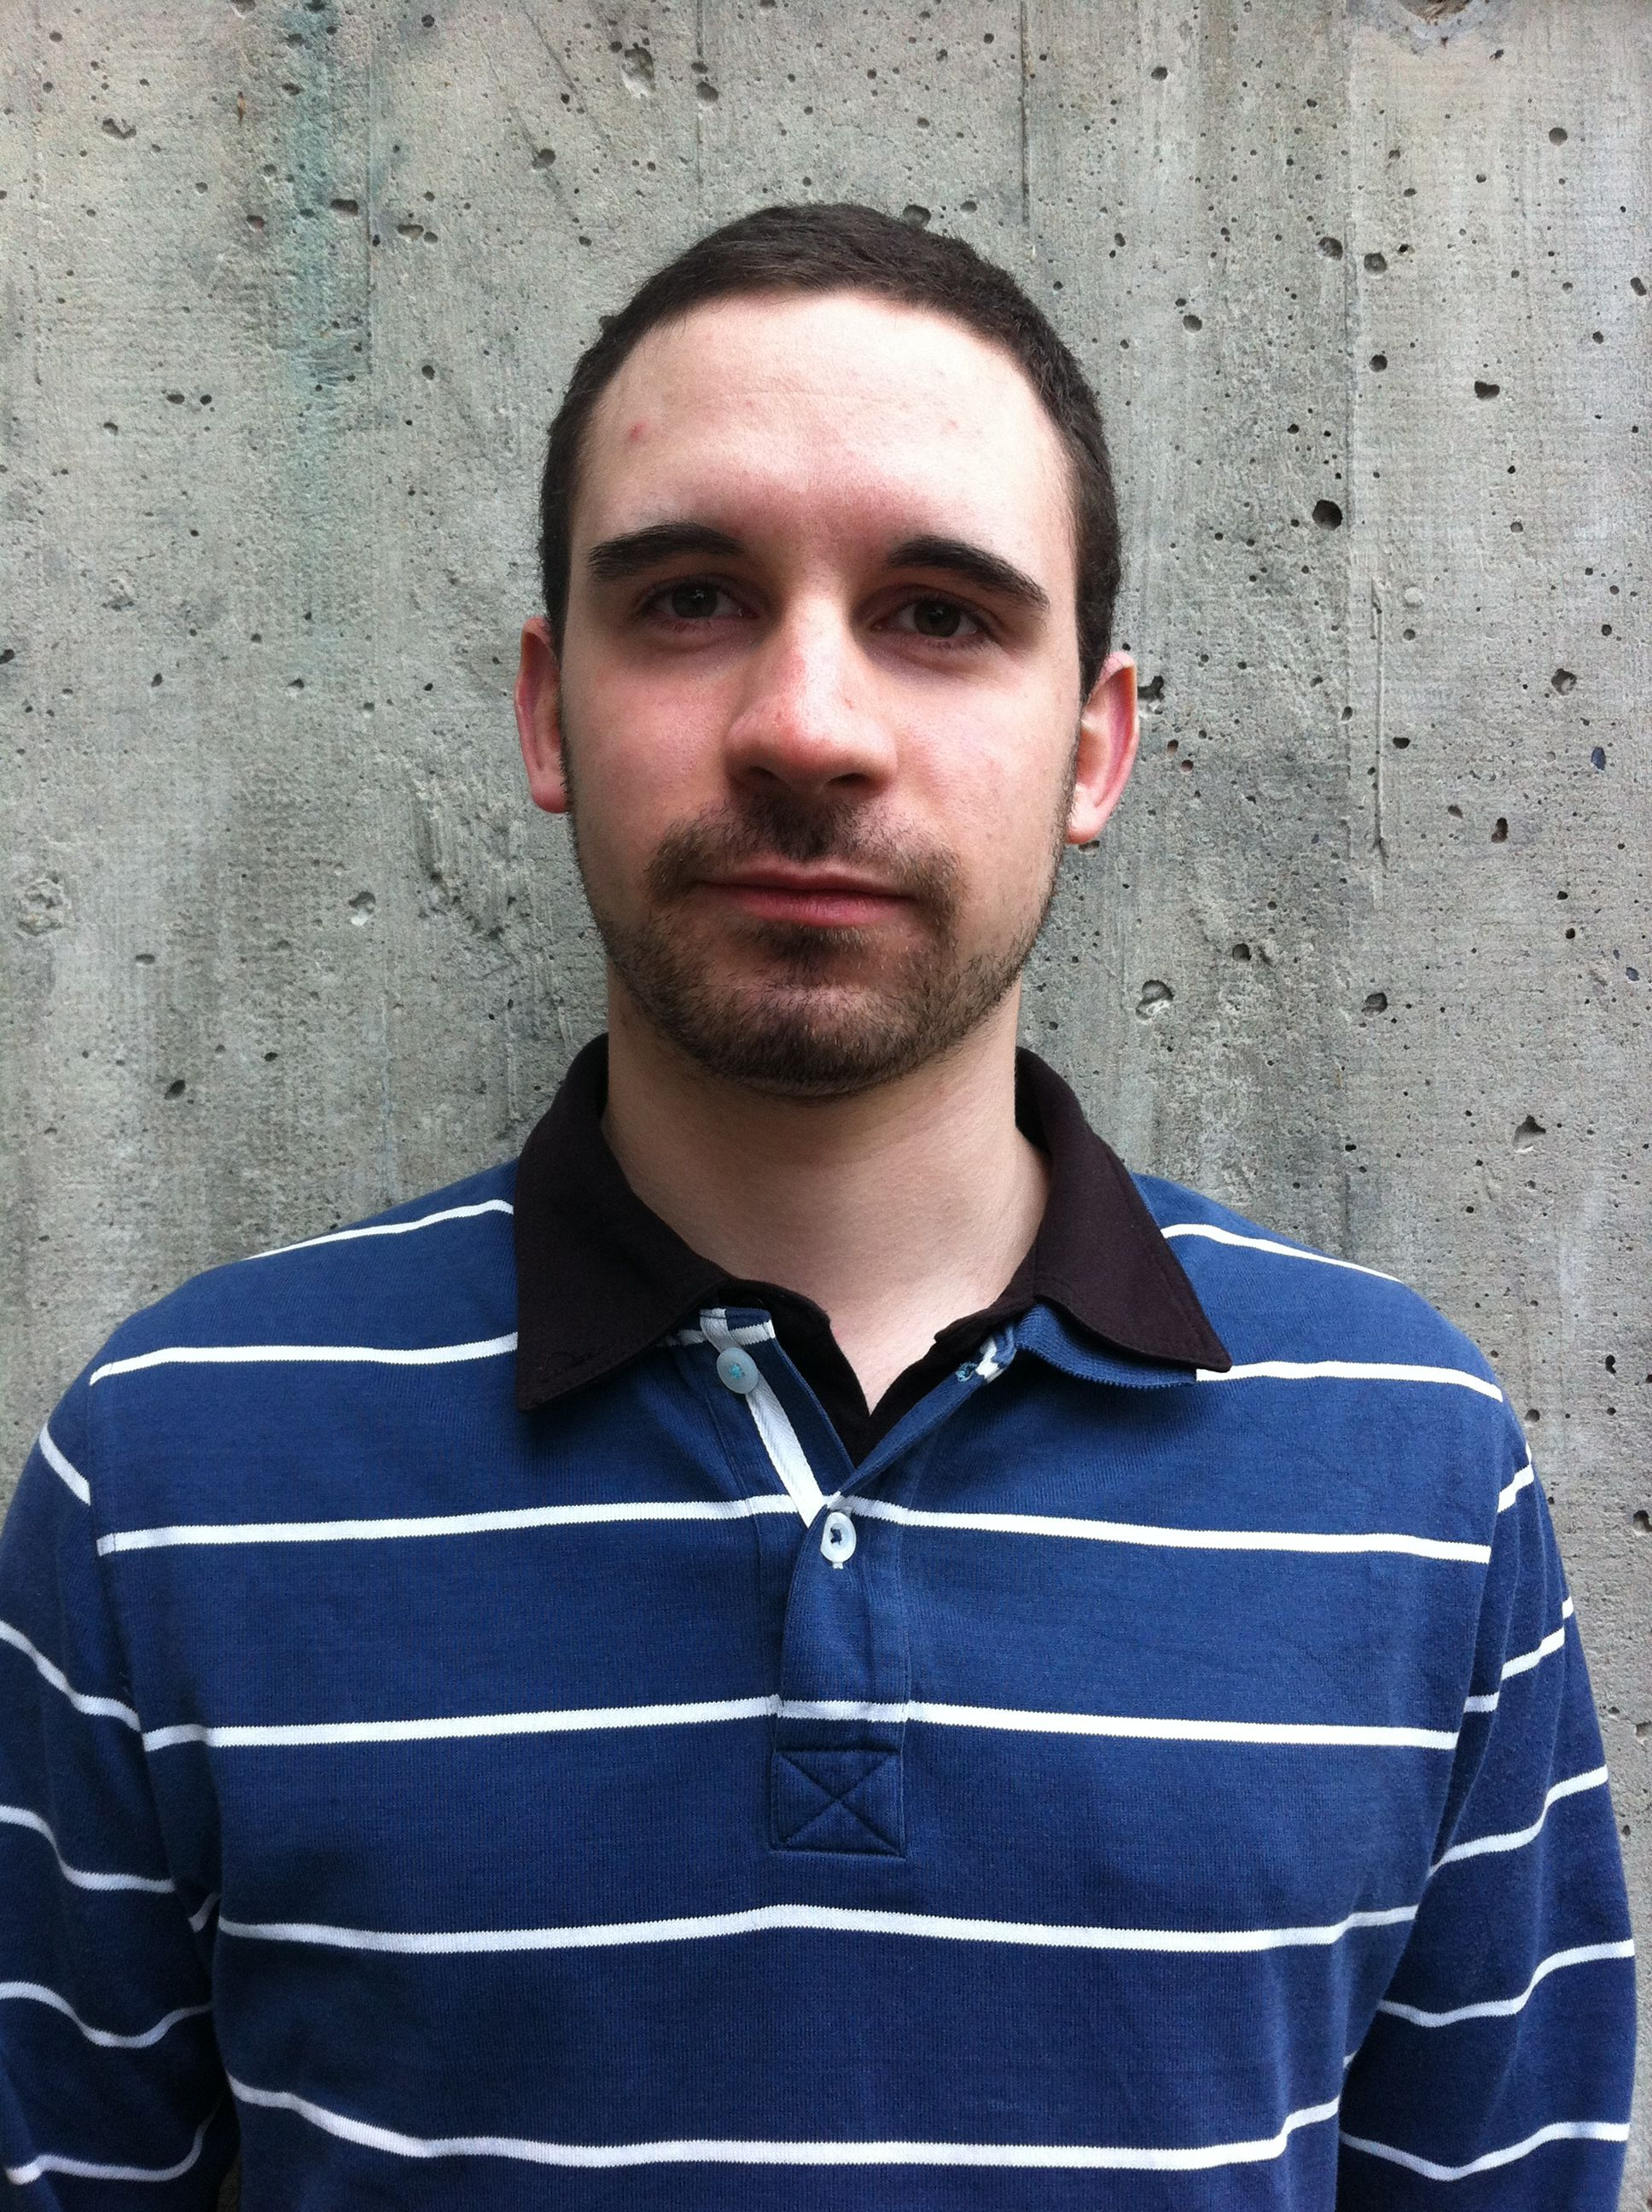
\includegraphics[width=0.3\textwidth]{img/tobias.jpg}
	\centering
	\caption{Tobias Blaser}
	\label{fig:tobias}
\end{figure}

\subsection*{Beat Gutzwiller}
\begin{figure}[H]
	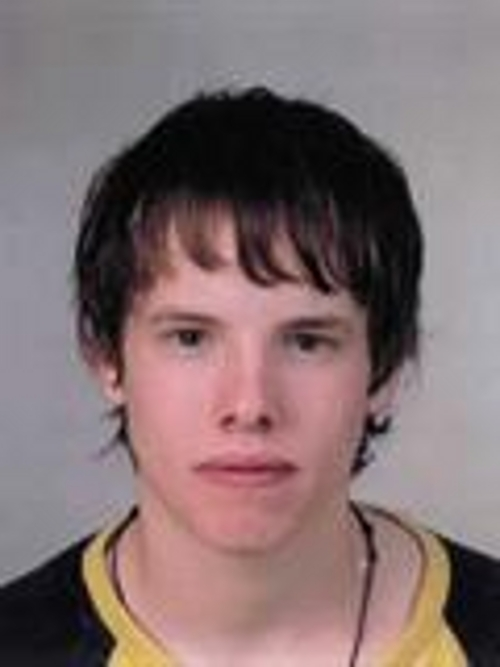
\includegraphics[width=0.3\textwidth]{img/beat.jpg}
	\centering
	\caption{Beat Gutzwiller}
	\label{fig:beat}
\end{figure}

\section{Externe Schnittstellen}
\teacher\ betreut die Semester Arbeit und begleitet das Team durch regelmässige Meetings.

%\chapter{Managementabläufe}
\section{Kostenvoranschlag}
Das Projekt dauert vom 21. Februar bis 31. Mai 2012 und ist mit 120 Stunden Aufwand pro Teammitglied veranschlagt. Dies macht eine Gesamtarbeitszeit von $$3 \cdot 120h=360h$$ Arbeitsstunden und bei einem Stundensatz von 110 Franken pro Stunde ergibt dies Kosten von $$360h \cdot 110CHF/h=39'600CHF$$ Weitere Ressourcen werden während der Entwicklungszeit nicht benötigt, der Test- und Implementierungsserver wird uns von der Hochschule Rapperswil zur Verfügung gestellt. Auch Kosten wie Anfahrtswege und Ähnliches wurden bewusst weggelassen, da diese im ``normalen`` Studienbetrieb ohnehin anfallen.
Dies ergibt eine durchschnittliche Arbeitszeit von $$\frac{120h}{14W} \simeq 8.5h/W$$ Stunden pro Woche pro Person damit das Projekt rechtzeitig beendet werden kann.

\section{Phasen}
Im Folgenden werden die einzelne Projektabschnitte in einer Übersicht dargestellt, die genauen Einzelschritte und Arbeitspakete der Phasen sind in Redmine erfasst. (Siehe Redmine-Zugang, im Abschnitt \ref{text:redmine} auf Seite \pageref{text:redmine})
\subsection{Inception}
Die Inception beinhaltet in erster Linie eine Idee. Diese wird im Projektantrag formuliert und mit Genehmigung desselben wird die Freigabe für diesen Projektplan erstellt. Während der Inception werden die Arbeitswerkzeuge eingerichtet, die Projektmitglieder als Team organisiert und deren Aufgaben festgelegt. Die Inception wird mit dem Meilenstein 1 (siehe \ref{text:milestone1}) abgeschlossen.
\subsection{Elaboration}
\subsubsection{Iteration 1}
In der ersten Iteration wird der Projektplan gemäss den Ergebnissen der Review überarbeitet. Danach folgt die genaue Ausarbeitung der Use-Cases, des Domainmodells, der Operation Contracts und Ähnlichem.
\subsubsection{Iteration 2}
Während der zweiten Iteration werden die Use-Cases detaillierter (``fully-dressed``) verfasst. Die logische Architektur und das Java-Klassenmodell werden entworfen. Das Ende der Elaboration ist zeitgleich mit dem Meilenstein 3 (siehe \ref{text:milestone3}). 
\subsection{Construction}
\subsubsection{Iteration 1}
Construction ist die Hauptimplementierungsphase. In dieser Zeit werden die während der Elaboration ausgearbeiteten Klassen implementiert und passende Unit-Tests (mithilfe von JUnit 4) ausgearbeitet.
\subsubsection{Iteration 2}
Die zweite Konstruktions-Iteration befasst sich nebst den restlichen Implementierungen mit Usability Tests und Bugfixing.
\subsubsection{Iteration 3}
Die dritte und letzte Iteration befasst sich mit dem Feinschliff. Dazu gehört weiteres Bugfixing und Systemtests. Gegen Ende dieser Iteration erfolgt ein ``Code-Freeze`` in dem kein weiteres Feature mehr hinzugefügt werden darf und nur noch Verbesserungen auf Bug-Ebene erlaubt sind. Siehe dazu auch Meilenstein 4 (Abschnitt \ref{text:milestone4})
\subsection{Transition}
Die Abschlussphase. In dieser geht es Hauptsächlich um die Erstellung der Benutzerdokumentation und die Vorbereitungen für die Schlusspräsentation. Sie wird dann auch vom Meilenstein 5 (siehe \ref{text:finish}) abgeschlossen.
\section{Meilensteine}
\subsection{Review Projektplan}
\label{text:milestone1}
Termin: 8. März 2012 13:10 Uhr \\
Review Projektplan mit Zeitplan und aktuellen Iterationsplänen\\
Der Projektplan wurde zu dem Zeitpunkt bereits abgegeben und an diesem Termin mit dem Betreuer besprochen. Nach erfolgtem Review verläuft das weitere Projekt gemäss Projektplan.

\subsection{Anforderungen und Analyse}
Termin: 20. März 2012 14:05 Uhr \\
Review der Anforderungsspezifikation und der Domainanalyse\\
Zu diesem Zeitpunkt stehen das Domainmodell (als konzeptionelles Klassendiagramm) und sämtliche Use-Cases (im ``brief``-Format, die wichtigen ``fully-dressed``) fest. Die Soll-Szenarien sind bekannt und als ``Features`` im Redmine erfasst.
\subsection{Ende Elaboration}
\label{text:milestone3}
Termin: 3. April 2012 14:05 Uhr \\
Zwischenpräsentation mit Demo eines Architekturprototypen, Review\\

\subsection{Erster lauffähiger Prototyp}
Termin: 3. April 2012 \\
Zu diesem Zeitpunkt existiert eine rudimentäre Version der Software die die Core-Funktionalität besitzt, soll heissen min ein lauffähiger Test, Fetchen der Website funktioniert und es wird ein Report (z.B. auf stdout) angezeigt
Dieser Meilenstein fällt mit dem Milestone ``Ende Elaboration`` zusammen.

\subsection{Architektur \& Design}
\label{text:architecture}
Termin: 24. April 2012 14:05 Uhr \\
Review von Architektur/Design und Architekturdokumentation\\

\subsection{Codefreeze}
\label{text:milestone4}
Termin: 18. April 2012 23:59 Uhr \\
Software soll soweit ``fertig`` sein. Es werden keine neuen Features mehr implementiert, nur noch Bugfixing betrieben. Zehn Tage Puffer soll zum Vollenden der Doku und Vorbereiten der Schlusspräsentation genutzt werden.

\subsection{Schlusspräsentation}
\label{text:finish}
Termin: 29. Mai 13:00 Uhr \\
Präsentation und Demo der Software\\

\section{Besprechungen}
Das Team trifft sich regelmässig jeweils am Dienstagnachmittag von 13:10 bis 16:50 Uhr im dem im Übungsraum \room, um sowohl den aktuellen Stand der Dinge zu besprechen als auch gemeinsame Tätigkeiten wie das Domain- und Klassenmodell auszuarbeiten durchzuführen. Die eventuell übrig bleibende Zeit wird von den Teammitgliedern individuell genutzt, um das Projekt in den ihnen zugewiesenen Aufgabenbereichen voranzutreiben.

%\chapter{Risikomanagement}
\section{Risiken}

Im Folgenden werden die zu erwartenden Risiken aufgeführt und Massnahmen im Falle deren Eintretens gezeigt. Die akkumulierte Reservezeit aller gewichteten Risikoschäden beläuft sich auf 
24 Stunden.

\begin{table}[h!]
	\centering
	%Die Spalten werden aufgeteilt auf 0.3 resp. 0.7-fache Textbreite
	\begin{tabular}{|p{0.3\textwidth} | p{0.7\textwidth} |}
	\hline	
	Risiko-ID & 1 \\
	\hline
	Titel & Implementierungshindernis \\
	Beschreibung & Aufgrund einer nicht bedachten Schwierigkeit, verzögert sich die Entwicklung des Programms \\
	max. Schaden	& 10h \\
	Eintrittswahrscheinlichkeit & 0.4 \\
	Gewichteter Schaden	& 4h \\
	Vorbeugung	& Sorgfältige Abklärungen im Vorfeld der Implementierung \\
	Massnahmen	& Zusätzliche Entwicklungszeit, um das Problem zu lösen \\
	\hline
	\end{tabular}
\end{table}

\begin{table}[h!]
	\centering
	\begin{tabular}{|p{0.3\textwidth} | p{0.7\textwidth} |}
	\hline
	Risiko-ID & 2 \\
	\hline
	Titel & Fehleinschätzung \\
	Beschreibung & Der Zeitaufwand für einzelne Arbeitspakete wurde falsch eingeschätzt \\
	max. Schaden	& 15h \\
	Eintrittswahrscheinlichkeit & 0.6 \\
	Gewichteter Schaden	& 9h \\
	Vorbeugung	& Aufwand für die Pakete wird im Team geschätzt um einen optimalen Schätzwert zu erhalten \\
	Massnahmen	& Kritische Arbeitspakete werden zuerst bearbeitet, optionale Features dann nach Möglichkeit implementiert \\
	\hline	
	\end{tabular}
\end{table}

\begin{table}[h!]
	\centering
	\begin{tabular}{|p{0.3\textwidth} | p{0.7\textwidth} |}
	\hline
	Risiko-ID & 3 \\
	\hline
	Titel & Performance \\
	Beschreibung & Das Abrufen der Website kann nicht in nützlicher Frist durchgeführt werden\\
	max. Schaden	& 50h \\
	Eintrittswahrscheinlichkeit & 0.2 \\
	Gewichteter Schaden	& 10h\\
	Vorbeugung	& Es wird von Anfang an möglichst ressourcenschonend programmiert \\
	Massnahmen	& Optimierung der Algorithmen\\
	\hline	
	\end{tabular}
\end{table}

\begin{table}[h!]
	\centering
	\begin{tabular}{|p{0.3\textwidth} | p{0.7\textwidth} |}
	\hline
	Risiko-ID & 4 \\
	\hline
	Titel & Webserver blockieren Serienabfragen \\
	Beschreibung & Es kann sein, das einzelne Webserver unseren Client blockieren wenn zu viele Anfragen in zu kurzer Zeit erfolgen \\
	max. Schaden	& 10h \\
	Eintrittswahrscheinlichkeit & 0.1 \\
	Gewichteter Schaden	& 1h \\
	Vorbeugung	& Alternativszenario mit zeitverzögerten Abfragen wird in Betracht gezogen \\
	Massnahmen	& Obiges Szenario wird anstelle der schnellstmöglichen Abfragegeschwindigkeit implementiert \\
	\hline	
	\end{tabular}
\end{table}

\begin{table}[h!]
	\centering
	\begin{tabular}{|p{0.3\textwidth} | p{0.7\textwidth} |}
	\hline
	Risiko-ID & 5 \\
	\hline
	Titel & Pluginarchitektur \\
	Beschreibung & Ob und wie eine Pluginarchitektur unter Java funktioniert ist unbekannt. \\
	max. Schaden	& Projektfehlschlag 120h \\
	Eintrittswahrscheinlichkeit & 0.1 \\
	Gewichteter Schaden	& 12h \\
	Vorbeugung	& Funktion einer Pluginarchitektur unter Java frühzeitig abklären. \\
	Massnahmen	& Grundsätzliche Funktion vor weiterer Planung abklären. \\
	\hline	
	\end{tabular}
\end{table}

\clearpage	

\section{Umgang mit Risiken}
Das Projektteam wurde über sämtliche oben erfassten Risiken informiert und ist sich über die zu ergreifenden Massnahmen im Schadenfall im Klaren.
Weitere, in der Evaluierung übersehene Risiken und deren Schäden, werden im Falle deren Auftretens vom Gesamtteam behandelt und ausgebessert.

%\chapter{Arbeitspakete}
Die einzelnen Arbeitspakete werden Mithilfe vom Projektverwaltungstools Redmine organisiert. Für die Betreuer wurde ein eigener Zugang zum Redmine-Projekt eingerichtet.
Genauere Informationen zum Redmine-Zugang, siehe Abschnitt \ref{text:redmine}
%\chapter{Infrastruktur}

\section{Entwicklung}
Erforderliche Hard- und Software:
\begin{itemize}
	\setlength{\itemsep}{-\parsep}
	\item Persönliche Entwicklungsgeräte für jedes Teammitglied, bevorzugt Laptop
	\item Entwicklungsumgebung
	\item \ac{SVN} Server
	\item Redmine Projektmanagement Tool
	\item Tex-Editor oder Tex-Suite inkl. Vorschau (z.B. Gummi) zum Verfassen der Dokumentation
	\item Tex-Umgebung zum kompilieren der Tex-Files
\end{itemize}

\subsection{Entwicklungsumgebung}
Zum Entwickeln wird eine Entwicklungsumgebung, bevorzugt Eclipse oder eine darauf aufbauende Umgebung benötigt. Die Entwicklungsumgebung soll folgende Anforderungen erfüllen:
\begin{itemize}
	\setlength{\itemsep}{-\parsep}
	\item Coding Unterstützung der Sprache Java
	\item Refactoring Tools
	\item Integrierte \ac{JVM}
	\item SVN Unterstützung
\end{itemize}

\subsection{SVN Server}
Zur Versionsverwaltung des Programmcodes und der Dokumentationsource wird ein externer Versionierungsserver benötigt. Die Dokumentation wird in \LaTeX\ verfasst, daher drängt es sich auf, die Tex-Sourcefiles ebenfalls zu versionieren. Bevorzug wird \ac{SVN}, weil das Projektteam die Integration in Eclipse bereits kennt und mit dem entsprechenden Eclipse Plugin Erfahrungen besitzt.

\subsection{Projektmanagement Tool}
Zur Koordination des Projekts und der Vereinfachung der Zusammenarbeit wird Redmine verwendet. SVN wird in Redmine eingebunden, sodass auch über Redmine direkt auf das Repository zugegriffen werden kann und Zugriff auf die Sourcefiles der Dokumentation besteht.

\section{Betrieb}
Zum Betrieb von "<PhipS"> werden folgende Geräte benötigt:
\begin{itemize}
	\setlength{\itemsep}{-\parsep}
	\item Desktop-Rechner mit JVM Version 1.6 oder 1.7 sowie einer Internetverbindung.
	\item Repository-Server
\end{itemize}

\subsection{Ausführungsplattform}
Zum Ausführen von "<PhipS"> wird ein Desktop Rechner mit einer JVM benötigt. Internetverbindung ist von Vorteil für den Zugriff auf Repositories oder das Analysieren von externen Webseiten. Auf dem Rechner sollten einige Megabyte Speicherplatz frei sein für die Applikation selbst und die Checks, die aus dem Repository heruntergeladen werden.

\subsection{Repository Server}
Nebst den selbst definierbaren Repositories wird es ein Standard-Repository für Checks geben. Dazu ist ein Repository Ordner auf einem allgemein zugänglichen Server nötig. Die Nutzer können direkt keine Checks hochladen, Lesezugriff ist ausreichend. Möchten Nutzer Checks andern Nutzern zur Verfügung stellen, so werden diese durch die Repositorybetreiber geprüft und von diesen Hochgeladen. Dazu wird ein \ac{SFTP} Client benötigt.


%\chapter{Qualitätsmassnahmen}

\section{Dokumentation}
Die Dokumentation wird in \LaTeX\ verfasst. Dies bietet wesentliche Vorteile:
\begin{itemize}
	\setlength{\itemsep}{-\parsep}
	\item Plaintextsourcefiles, die mit SVN versioniert und bei unterschiedlichen Zuständen problemlos zusammengeführt werden können
	\item Wenig Speicherplatzverbrauch durch die Sourcefiles
	\item Durch den Verzicht auf eine Office Umgebung ist die Wahrscheinlichkeit eines Absturzes und eine Beschädigung der Dateien geringer
	\item Das Projektteam muss keine unnötige Zeit für Layouting mit einem Office Programm und die damit verbundenen Probleme verwenden oder ein Desktop Publishing Programm einsetzen. Dank einer ausgereiften Vorlage wird der Layoutingaufwand mit \LaTeX\ klein gehalten.
	\item Das Projektteam kann die Dokumentation aufteilen und die einzelnen Teile in die Hauptdatei einbinden.
\end{itemize}
Die Qualität wird dadurch sichergestellt, dass jedes Projektmitglied die Qualität für die von ihm produzierten Teilstücke gewährleistet und gleichzeitig die Dokumentation als Ganzes vom gesamten Team überprüft wird. Der Projektleiter gewährleistet, dass keine Teilbereiche bei der Abgabe fehlen.

\section{Projektmanagement}
Zur Unterstützung des Projektmanagements wird Redmine mit SVN Anbindung eingesetzt. Verwaltet werden sollen Arbeitspakete, Meilensteine, Einteilung von Teammitgliedern, Projektstand und Projektenwicklung.

\subsection{Gastzugang Redmine}
\label{text:redmine}
Zugang: http://152.96.56.72/redmine/\\
Benutzer: supervisor\\
Passwort: supervisor \\

Der Supervisor hat die Rechte um alle Beiträge, Tickets, Dokumente, sowie den Kalender und die Gantt-Chart einzusehen und nötigenfalls zu kommentieren, jedoch keinerlei Schreib- oder Verwaltungsrechte.

\section{Entwicklung}
Der Programmcode wird mit SVN versioniert. Die Qualität soll einerseits durch den entsprechenden Entwickler selbst, andererseits durch Reviews, Struktur Checks und Funktionstests gewährleistet werden.

\subsection{Vorgehen}
Bei der Entwicklung wird nach dem RUP vorgegangen. Insbesondere liegt das Augenmerk auf einer iterativen und agilen Entwicklung. Für bekannte Probleme sollen standardisierte Software Patterns angewendet werden. Auch die Prinzipien der GoF sollen in die Entwicklung einfliessen.

\subsection{Unit Testing}
Das Zusammenwirken der Klassen, insbesondere die Interaktion mit dem Repositoryserver und die Kommunikation mit einer beliebigen Webseite sollen durch Unit Tests überprüft werden. Zudem soll jeder Check verschiedene Unit Tests bestehen müssen.

\subsection{Code Reviews}
Jeder Programmteil soll Reviews unterzogen werden. Das Hauptaugenmerk bei den Reviews liegt auf Pre-/Postconditions, unerlaubten und unerwarteten Werten, Seiteneffekten sowie dem Einhalten der Code Style Guidelines.
Die Reviews werden ohne den betreffenden Programmierer stattfinden, um zu verhindern, dass ein "Vorstellen / Erklären"\ des Codes durch den Entwickler stattfindet. Programmcode und zugehörige Kommentare müssen selbsterklärend aufgebaut sein.

\subsection{Code Style Guidelines}
Für die Entwicklung sollen die Oracle Code Style Conventions angewendet werden: \\ \href{http://www.oracle.com/technetwork/java/codeconv-138413.html}{www.oracle.com/technetwork/java/codeconv-138413.html}

\section{Testen}

\subsection{Testumgebung}
Als Testumgebung soll von Hand ein HTML-Seiten Gerüst aufgebaut werden. Jede Seite enthält eine Anzahl verschiedener Fehler. Getestet wird, ob und wie gut die Applikation die Fehler erkennt. Die Fehler sollen von verschiedenen Schwierigkeitsgraden sein.

\subsection{Unit Tests}
Die Kernfunktionalitäten sollen mit Unit Tests überprüft werden. Getestet wird mit JUnit 4. Gearbeitet wird mit je drei Tests pro Testszenario.

\subsubsection{Was soll getestet werden}
Klassen, die Funktionen besitzen, die über Setter und Getter hinausgehen müssen getestet werden. Es sollen alle Methoden getestet werden, die mehr als fünf Zeilen lang sind und funktional mehr als ein Setter oder ein Getter ausführen. 

\subsubsection{Wie soll getestet werden}
Die Funktion der entsprechenden Methoden soll mit einem Normalfall, Fehlerfall und einem oder mehreren Randfällen getestet werden.

\subsection{Pluginchecks}
Jedes Plugin muss einige Tests bestehen, damit das korrekte Zusammenarbeiten mit der Applikation gewährleistet werden kann. Getestet werden soll, ob das Plugin korrekt angesprochen werden kann und ein korrektes Resultat in der vorgeschriebenen Form liefert. Zusätzlich soll mit drei Testszenarien, den Fähigkeiten des Plugins entsprechend, die Funktionalität überprüft werden. Die Szenarien testen den Normalfall, den Fehlerfall und einen oder mehrere Randfälle.

\subsection{Usability Test}
Die Benutzbarkeit der grafischen Oberfläche soll mittels Usability Test mit drei Testpersonen überprüft werden.

\subsection{WorstCase Test}
Getestet werden sollen Worst Case Szenarien, unabhängig der Klasse: 
\begin{itemize}
	\setlength{\itemsep}{-\parsep}
	\item Keine Internetverbindung vorhanden
	\item Angegebenes Repository fehlerhaft oder nicht vorhanden
	\item Plugin defekt
	\item Fehlen der Settings-Datei
	\item Zu checkende Seite, die grösser als der Arbeitsspeicher ist
	\item Sehr langsame Internetverbindung
\end{itemize}
Keiner der angegebenen Fälle darf das Programm zum Absturz bringen. Ausserdem sollen die Fehler in jeder Situation zuverlässig geloggt werden.
Pro Konfiguration sollen drei Tests durchgeführt werden.

\subsection{Systemtest}
Das System soll mit zehn verschiedenen, realitätsnahen Szenarien als ganzen getestet werden (Blackboxtest). 


\end{document}
